\documentclass[polish,edition=2024]{zpiday}
\usepackage{csvsimple}
\usepackage{graphicx}
\usepackage{subcaption}
\usepackage{forest}
\usepackage{listings}

\usepackage{lipsum}
\title{Metoda trójwymiarowego modelowania obszarów urbanistycznych z wykorzystaniem metod fotogrametrii}
\acronym{URB3D}
\supervisor{dr hab. inż. Marek Krótkiewicz, prof. PWr}
\members{Daniel Borkowski \and Julia Farganus \and Rafał Mielniczuk \and Katarzyna Wochal}

\projectLogo{images/logo_white.png}


\begin{document}

\maketitle

\begin{abstract}
    Celem pracy jest wykonanie aplikacji, która wykorzystuje metody fotogrametrii do modelowania miejskich scen 3D. Dane wejściowe stanowią zdjęcia obszarów miejskich, które są przetwarzane w celu stworzenia modelu 3D, a następnie segmentowane na obiekty przestrzeni miejskiej, takie jak budynki, tereny zielone, itp.. Aplikacja będzie wizualizować model oraz wyniki segmentacji semantycznej.

    Innowacyjność tego projektu polega na połączeniu, adaptacji i udoskonaleniu najlepszych dostępnych rozwiązań, takich jak Gaussian Splatting i PointNet, aby stworzyć nowy, kompleksowy produkt.

    Przetwarzanie dużych scen miejskich jest wyzwaniem dla obecnie istniejących rozwiązań, które skupiają się głównie na pojedynczych obiektach lub zamkniętych scenach. Typowa scena miejska natomiast może obejmować setki zdjęć, a powstała chmura może zawierać miliony punktów. Dodatkowym wyzwaniem jest niezbalansowana reprezentacja kategorii semantycznych. Nasze rozwiązanie ma na celu efektywne przetwarzanie dużych zbiorów danych przy rozsądnym zużyciu zasobów czasowych i pamięciowych.

    Zastosowania biznesowe otrzymywanych w ten sposób modeli 3D są szerokie: od gier wideo, przez architekturę, robotykę, pojazdy autonomiczne, po modelowanie urbanistyczne.
\end{abstract}

\section{Wprowadzenie}
Nasz projekt skupia się na problemie rekonstrukcji trójwymiarowej scen urbanistycznych, jej klasyfikacji oraz wizualizacji. Warto podkreślić, że obszar naszej pracy jest relatywnie nowy i stawia wyzwania związane z efektywnością przetwarzania dużego zbioru danych - w naszym przypadku chmury punktów, która może składać się nawet z paru milionów punktów. Na rynku dostępne są rozwiązania które możemy wykorzystać, więc naszym głównym celem jest zbadanie ich użyteczności w naszym problemie i ich ewentualna adaptacja. 

Nasze rozwiązanie będzie umożliwiało przeprowadzenie rekonstrukcji do modelu trójwymiarowego na podstawie odpowiednio przygotowanego zbioru zdjęć, klasyfikację otrzymanej sceny na zbiór pre-definiowanych klas istotnych w kontekście scen urbanistycznych, oraz wizualizację wykonanych obliczeń. 

Jako zespół stawiamy następujące cele, które chcemy zrealizować:

\begin{enumerate}
    \item Skomponowanie własnego zbioru danych 
    \item Wykorzystanie algorytmu Gaussian Splatting do rekonstrukcji sceny 3D
    \item Filtracja chmury punktów przy użyciu różnych technik 
    \item Zastosowanie architektur sieci neuronowych takich jak PointNet do klasyfikacji chmury punktów 
    \item Adaptacja istniejących bibliotek do wizualizacji wyników 
    \item Implementacja własnego algotymu do renderowania gaussianów
\end{enumerate}

\subsection{Stan wiedzy}

Unikalność naszego projektu wynika z połączenia wielu rozwiązań które istnieją samodzielnie na rynku. Alogrytm Structure-from-Motion jest popularną fotogrametryczną techniką otrzymywania chmury punktów ze zbioru zdjęć i jego implementacja oferowana jest m. in. przez oprogramowanie COLMAP. W przypadku modelu 3D można napotkać różne adaptacje algorytmu Gaussian Splatting, jak np. CityGaussian .... Ważnym krokiem jest również filtracja chmury punktów w celu usunięcia odstających punktów lub tych nieistotnych dla wyników klasyfikacji.  

\textbf{Wykorzystane oprogramowanie}
z fiszki można wrzucić 

\section{Wyniki}

\subsection{Funkcjonalność oprogramowania}

Modularność naszego projektu sprawia, że wygodniej jest omówić niezależnie każdą z części. Dla jasności, przebieg całego procesu jest następujący:
\begin{enumerate}
    \item Wczytanie plików zdjęć.
    \item Rekonstrukcja SFM do chmury punktów, która jest podstawą do kolejnego etapu.
    \item Wytrenowanie modelu sceny przy pomocy algorytmu Gaussian Splatting.
    \item Filtracja, następnie segmentacja chmury punktów z poprzedniego kroku.
\end{enumerate}
Każda funkcjonalność, jak i wizualizacje wyników poszczególnych zadań są dostępne poprzez interfejs użytkownika. 

\subsection{Akwizycja danych}
W projekcie założono wykorzystanie metod fotogrametrycznych do tworzenia trójwymiarowych modeli obszarów urbanistycznych. Za część projektu przyjęto z tego względu również pozyskanie własnych
zestawów danych fotograficznych (fotogramów), które spełniałyby wymogi techniczne, umożliwiające
późniejszą rekonstrukcję 3D. Wynikowe zbiory zdjęć powstały poprzez wykonanie dużej liczby ujęć, obejmujących wiele kątów i perspektyw oraz zapewniając odpowiednie nakładanie się obrazów dla poprawnego działania oprogramowania fotogrametrycznego.


Akwizycję zrealizowano na kampusie Politechniki Wrocławskiej, koncentrując się na budynkach C5,
C7 oraz Strefie Kultury Studenckiej (SKS)[\ref{fig:four-photos}] i pozyskując zdjęcia zarówno z lotów bezzałogowym statkiem powietrznym, jak i z poziomu gruntu. W jej wyniku przygotowano własne kompletne zbiory danych, które spełniły wymogi jakościowe i posłużyły do budowy testowych modeli.

\begin{figure}[h!]
    \centering
    \begin{minipage}{0.24\textwidth}
        \centering
        \includegraphics[width=\textwidth]{img/sks_dataset_1.jpg}
    \end{minipage}
    \hfill
    \begin{minipage}{0.24\textwidth}
        \centering
        \includegraphics[width=\textwidth]{img/sks_dataset_2.jpg}
    \end{minipage}
    \hfill
    \begin{minipage}{0.24\textwidth}
        \centering
        \includegraphics[width=\textwidth]{img/sks_dataset_3.jpg}
    \end{minipage}
    \hfill
    \begin{minipage}{0.24\textwidth}
        \centering
        \includegraphics[width=\textwidth]{img/sks_dataset_4.jpg}
    \end{minipage}
    \caption{Przykładowe zdjęcia z akwizycji danych przedstawiające SKS}
    \label{fig:four-photos}
\end{figure}

\subsubsection{Structure from motion}
Jedną z funkcjonalności oferowanych przez przygotowane oprogramowanie jest wyznaczanie struktury przestrzennej sceny w postaci chmury punktów na podstawie zbioru fotogramów przy pomocy techniki Structure from motion. Zaproponowana implementacja opiera się na wykorzystaniu popularnego narzędzia COLMAP\cite{schoenberger2016mvs}\cite{Schonberger_2016_CVPR}, które zostało włączone do projektu w postaci pythonowej biblioteki \href{https://github.com/colmap/pycolmap}{\textit{pycolmap}}. Biblioteka ta oferuje szereg funkcji umożliwiających przeprowadzenie kluczowych etapów procesu SfM, w tym wykorzystane w projekcie funkcjonalności do wykrywania cech charakterystycznych na obrazach, dopasowywania punktów wspólnych między obrazami czy przeprowadzania inkrementalnej rekonstrukcji, która dodatkowo została skonfigurowana za pomocą parametrów dobranych tak, aby zapewnić zadowalającą jakość wyniku przy zachowaniu wydajności.

W wyniku działania tak zaimplementowanego procesu powstają pliki binarne zapisujące dane przede wszystkim wyznaczonych punktów 3D i pozycji kamer. Biblioteka \textit{pycolmap} umożliwiła dodatkowo łatwe wprowadzenie funkcjonalności eksportu wyników do formatu PLY, którego to formatu plik zostaje wykorzystany do wizualizacji wygenerowanej chmury punktów. Z kolei reprezentacja w postaci plików binarnych zostaje w kolejnych etapach wczytywana i po przefiltrowaniu służy za podstawę do modelowania z zastosowaniem algorytmu Gaussian Splatting.

\begin{figure}[!ht]
  \centering
  \includegraphics[width=0.9\linewidth]{img/sfm_projection.png}
  \caption{Projekcja przykładowej chmury punktów na płaszczyznę porównana do zdjęcia}
\end{figure}

\subsection{Gaussian Splatting}
Przy pomocy biblioteki \textit{gsplat}\cite{ye2024gsplatopensourcelibrarygaussian} zawierającej implementację \textit{Gaussian Splatting} w Pythonie wykonaliśmy eksperymenty polegające na uruchomeniu algorytmu dla różnych wartości hiperparametrów w celu znalezienia wartości, które prowadzą do jak najbardziej optymalnego procesu trenowania w kontekście czasu trwania i wykorzystania pamięci. 

Na wejściu algorytmu podawana jest otrzymywana w procesie rekonstrukcji chmura punktów, która jest bazą do dalszego dzielenia i powstawania "gaussianów", a ich parametry: pozycja, kolor, skala i rotacja są optymalizowane przy pomocy metody spadku wzdłuż gradientu. Metryki przyjęte do oceny jakości to SSIM (Structural Similarity Index Measure), PSNR (Peak Signal-to-Noise Ratio) oraz LPIPS (Learned Perceptual Image Patch Similarity).

W wyniku przeprowadzenia eksperymentów okazało się, że najważniejszymi sterującymi procesem parametrami są 
\begin{enumerate}
    \item Liczba Gaussianów: w przypadku scen urbanistycznych w celu oddania odpowieniej szczegółowości potrzebne jest parę milionów Gaussianów, dla naszych scen było to zwykle 3 mln.
    \item Strategia i częstość adaptacji: określają w jaki sposób oraz jak często dodawane i usuwane są Gaussiany. 
    \item Liczba iteracji: zwykle im dłużej trenowana jest scena tym lepsze wyniki otrzymujemy, jednak zależy to również od przyjętej strategii. Liczba ta wpływa bezpośrednio na czas trenowania, powinna wynieść nie mniej niż paręnaście tysięcy.
    \item Stopień zmiennych harmonicznych: wyrażają one kolor, im większy stopień tym lepsza jakość sceny, ale też zwiększone zużycie pamięci.  
\end{enumerate}

Poniżej przedstawione są przykładowe wizualizacje. Renderowania zostały wykonane przy pomocy biblioteki nerfview która również służy do wizualizacji splatów. Na poniższych rysunkach są od lewej do prawej: prawdziwe zdjęcie i widok modelu.

\begin{figure}[!h]
    \centering
    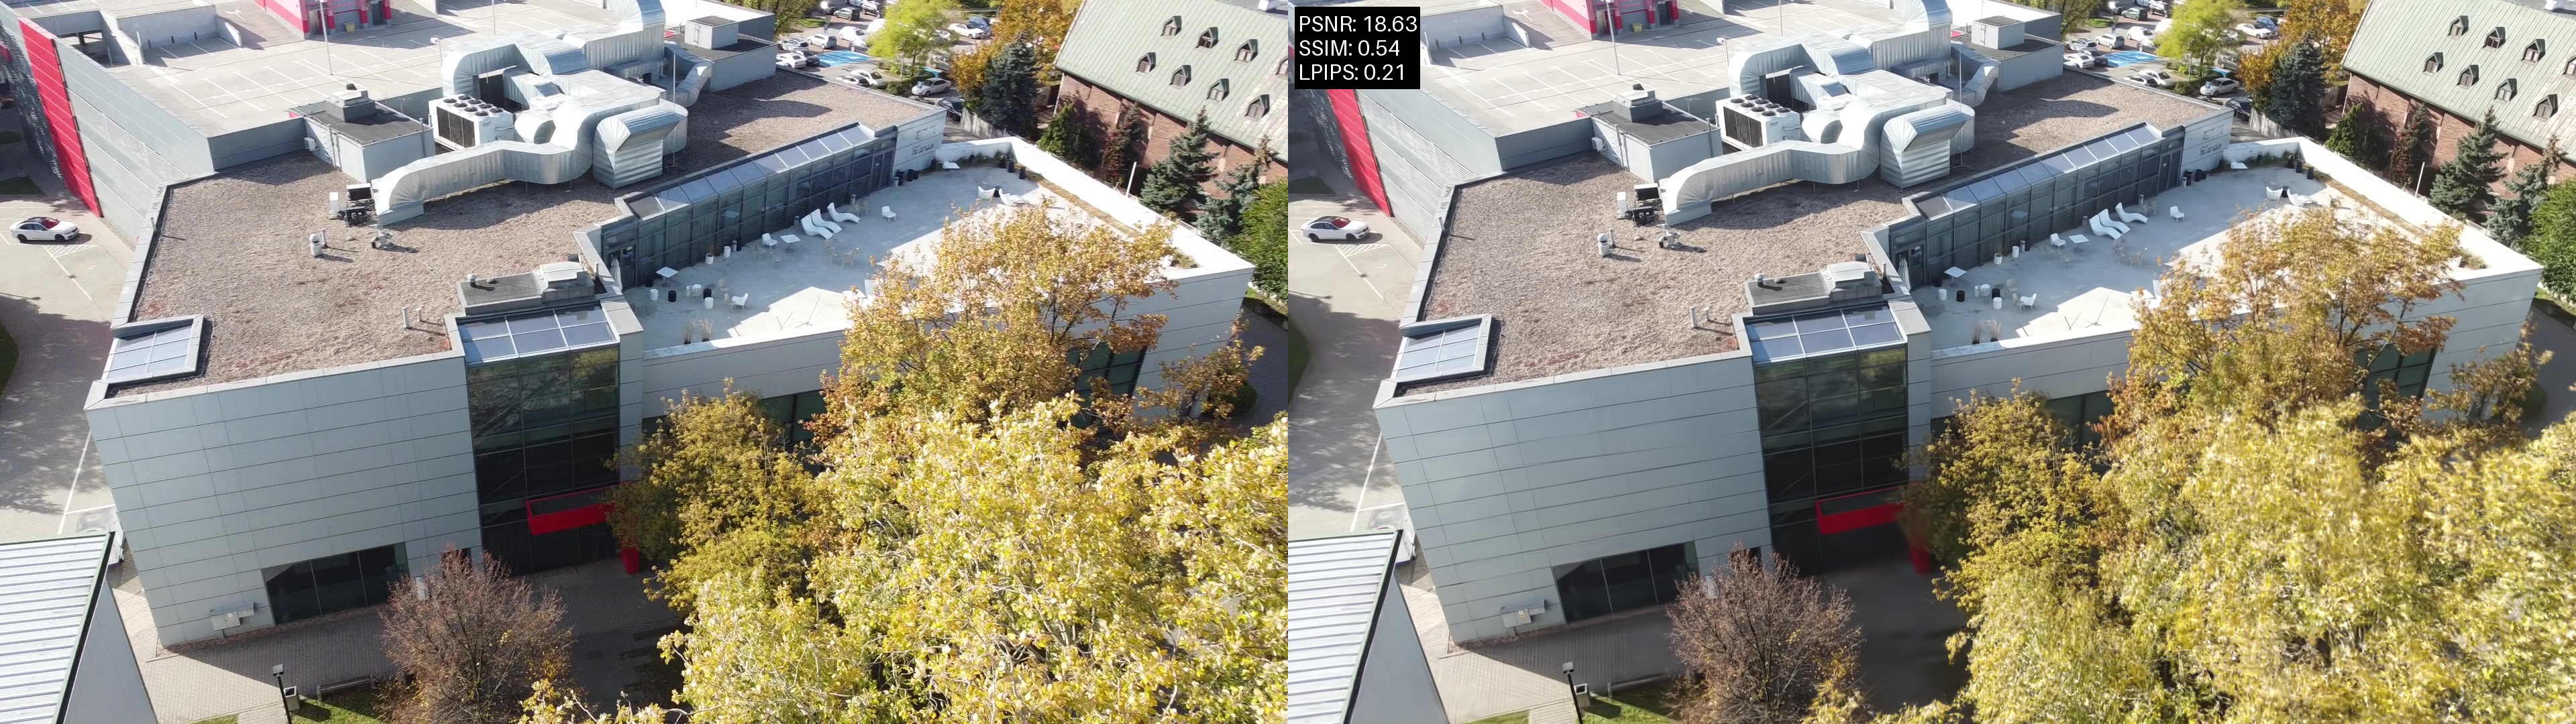
\includegraphics[width=1.0\linewidth]{images/sks_viper_0008.png}
    \caption{Scena SKS}
    \label{fig:sks_gs}
\end{figure}

\begin{figure}[!h]
    \centering
    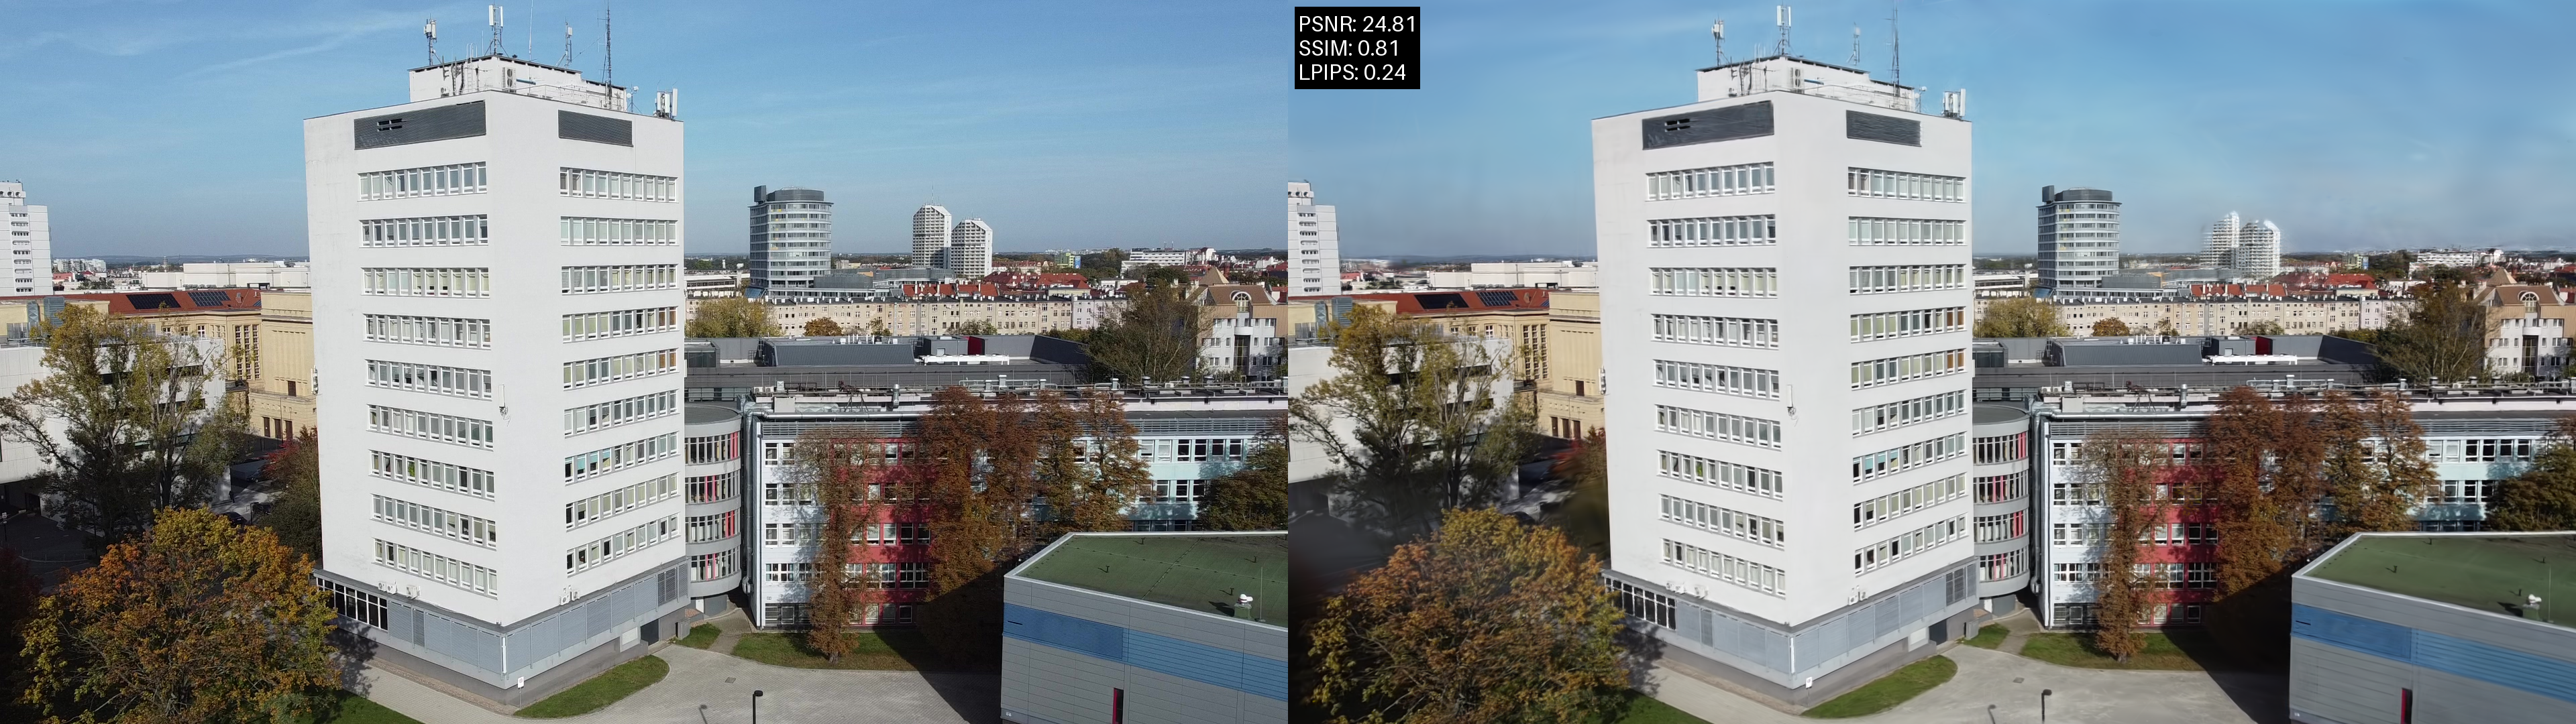
\includegraphics[width=1.0\linewidth]{images/c5_mouse_0001.png}
    \caption{Scena C5}
    \label{fig:c5_gs}
\end{figure}

\begin{figure}[!h]
    \centering
    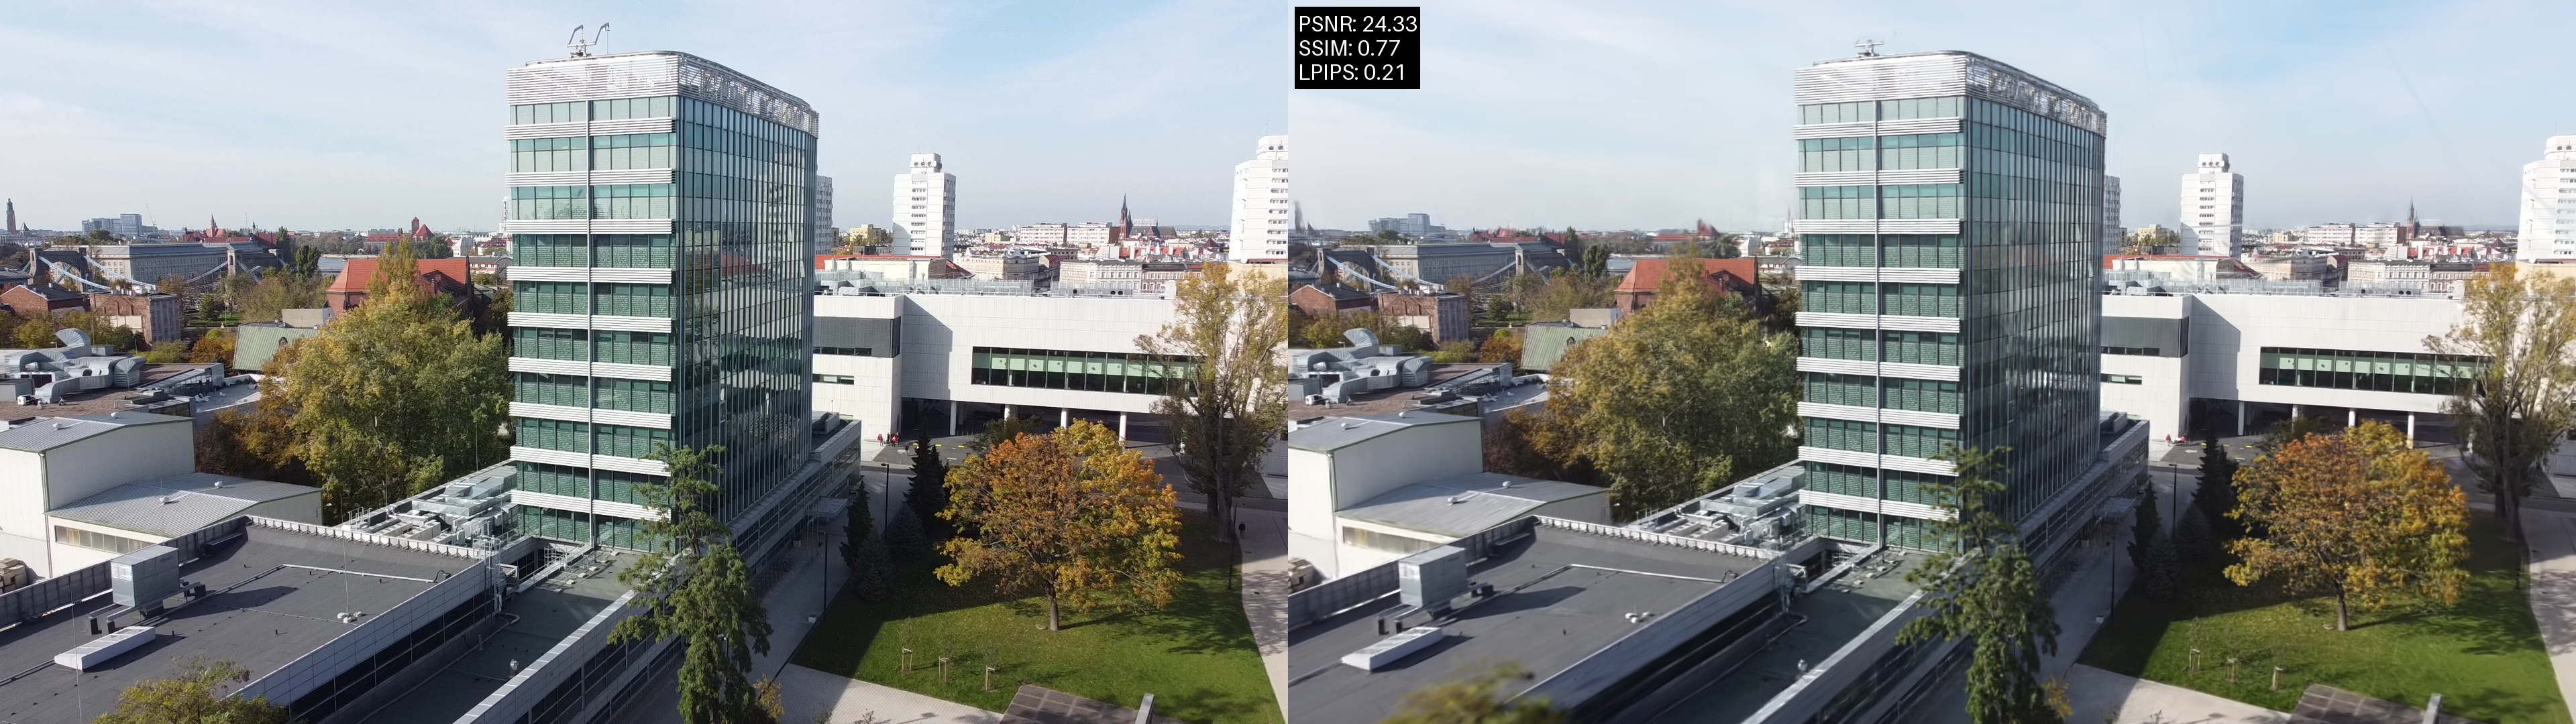
\includegraphics[width=1.0\linewidth]{images/c7_gepard_0006.png}
    \caption{Scena C7}
    \label{fig:c7_gs}
\end{figure}

\subsection{Segmentacja}
Używając biblioteki \textit{PyTorch} do uczenia głębokiego, w oparciu o istniejące rozwiązania i aktualny stan wiedzy, przygotowaliśmy i wytrenowaliśmy własne modele segmentacji semantycznej na chmurze punktów, otrzymanej w naszej aplikacji w wyniku działania poprzednich etapów i przekształceń na danych z nimi związanych. 
\textbf{Segmentacja semantyczna}
Zadanie postawione przed modelem jest jednym z kategorii zadań widzenia komputerowego. Polega ono na przypisaniu każdemu z punktów w chmurze etykiety określającej do jakiego rodzaju obiektu on przynależy, na przykład: czy jest on częścią budynku, drogi, samochodu, czy terenu zielonego. Obiektem wejścia jest zatem chmura punktów, natomiast na wyjściu otrzymujemy 

\subsection{Wizualizacja}
Wizualizacja modeli 3D stanowi wyzwanie dla użytkownika końcowego,
głównie z powodu braku spójnych platform umożliwiających realizację
całego procesu – od wgrania plików wejściowych po interakcję z modelem – w ramach jednej aplikacji.
Dostępne na rynku rozwiązania wymagają korzystania z aplikacji trzecich i pewnej wiedzy technicznej,
co prowadzi do problemów z integracją i spójnością działania.

Celem projektu było stworzenie intuicyjnego, dynamicznego i responsywnego \textbf{interfejsu} zintegrowanego z wydajnym \textbf{renderingiem} GPU.
Aplikacja umożliwia użytkownikowi końcowemu realizację pełnego procesu
wizualizacji – od tworzenia i modyfikacji modelu po jego segmentację i wyświetlanie – w jednej aplikacji.
Projekt rozwiązuje problem fragmentarycznej funkcjonalności dostępnych aplikacji, oferując spójne środowisko do obsługi modeli 3D.

\textbf{Korzyści z realizacji interfejsu}

\begin{itemize}
    \item zwiększona wydajność dzięki GPU,
    \item eliminacja konieczności korzystania z wielu narzędzi,
    \item uproszczony proces użytkowania, co zwiększa dostępność aplikacji dla mniej zaawansowanych użytkowników.
\end{itemize}

Rendering wykorzystuje plik .ply jako dane wejściowe do wczytania splatów.
Są one renderowane jako sześciany, w których wnętrzu generowane są shadery, bazujące na skalowaniu i rotacji splatów.
Takie podejście umożliwia abstrakcyjne przedstawienie splatów przy jednoczesnym zachowaniu wysokiej dokładności wizualnej.

Interfejs widoczny na ilustracji \ref{fig:ui} został zaimplementowany w \textit{QML}, \textit{PyQt}, natomiast rendering w technologiach \textit{C}, \textit{OpenGL} oraz \textit{OpenCL}, przedstawiony na zdjęciu \ref{fig:rendering}. Tymczasową wizualizację chmury wykonywaliśmy przy pomocy biblioteki \textit{VisPy}.


\begin{figure}[!ht]
    \centering
    \includegraphics[width=\textwidth]{images/UI-Rendering.png}
    \caption{Zrzut ekranu przedstawiający główny widok aplikacji}
    \label{fig:ui}
\end{figure}

\begin{figure}[!ht]
    \centering
    \includegraphics[width=\textwidth]{images/cloud_rendering.png}
    \caption{Zrzut ekranu przedstawiający własny renderer}
    \label{fig:rendering}
\end{figure}


\section{Podsumowanie}
Rekonstrukcja i klasyfikacja krajobrazów urbanistycznych ma wiele potencjalnych zastosowań w dziedzinach takich jak \textit{Smart City} czy też \textit{Virtual Reality}. Projekt "urb3d" pokazał, że wykonanie takiego oprogramowania jest możliwe przy pomocy integracji istniejących rozwiązań i ich adaptacji. 

\subsection{Wnioski}
Zaprojektowane oprogramowanie zapewnia intuicyjne korzystanie z funkcjonalności takich jak dostosowywanie parametrów, wczytywanie zdjęć, uruchamianie poszczególnych etapów oraz przeglądanie rezultatów. Odpowiednio dobrane algorytmy zapewniają jakościowe wyniki, które mogą być dalej wykorzystane razem lub oddzielnie. 

\subsection{Kierunki rozwoju}
W przyszłości projekt mógłby obejmować rekonstrukcję jeszcze większych obszarów urbanistycznych, co wiązałoby się z koniecznością zastosowania bardziej zaawansowanych technik optymalizacji. Warta wprowadzenia mogłaby okazać się kompresja danych w celu zmniejszenia końcowej liczby gaussianów w algorytmie \textit{splattingu}. Inny kierunek rozwoju to trenowanie modeli na różnych poziomach szczegółowości (ang. Level of Detail - LoD). Otwartym rozdziałem jest też testowanie kolejnych modeli segmentacji semantycznej i ich dostrajanie.

\subsection{Podziękowania}
Szczególne podziękowania należą się operatorce drona Paulinie, bez której z pewnością sukces w obszarze akwizycji danych nie byłby możliwy.

\bibliographystyle{plain}
\bibliography{references}


\end{document}